\documentclass{river-journal}
\usepackage{rivps}
%\usepackage[mtbold]{mathtime}

\usepackage{graphicx}
\usepackage{graphics}
\usepackage{subfigure}
\usepackage{cite}


%package added by author
\usepackage{tikz}
\usetikzlibrary{calc,positioning,arrows}
% for alternatives, see appendix of manual
\usepackage{url}
\usepackage{bibspacing}
\usepackage{rotating}


\newtheorem{guess}{Conjecture}

% bibliographies
\bibliographystyle{plain}
% also tested with natbib

\raggedbottom
\sloppy\par




\usepackage{etoolbox}
\patchcmd{\thebibliography}
  {\settowidth}
  {\setlength{\itemsep}{0pt plus 0.1pt}\settowidth}
  {}{}
\apptocmd{\thebibliography}
  {\small}
  {}{}


\begin{document}
\begin{opening}
\title{Privacy Enhanced Fast Mutual Authentication in 5G Network Using Identity Based Encryption}
\author{Mohsin Khan$^{*}$ and Valtteri Niemi}
\institute{Department of Computer Science\\
P.O. Box 68 (Gustaf Hällströmin katu 2b)\\
FI-00014 UNIVERSITY OF HELSINKI, FINLAND  \\
E-mail: \{mohsin.khan, valtteri.niemi\}@helsinki.fi\\
$^*$Corresponding Author}
\end{opening}

\runningtitle{Privacy Enhanced Fast Mutual Authentication}
\runningauthor{Mohsin Khan and Valtteri Niemi}

\subsection*{Abstract}
Subscription privacy of a user has been a historical concern with all the previous generation mobile networks, namely, GSM, UMTS, and LTE. While a little improvement have been achieved in securing the privacy of the long-term identity of a subscriber, the so called IMSI catchers are still in existence even in the LTE and advanced LTE networks. Proposals have been published to tackle this problem in 5G based on pseudonyms, and different public-key technologies. This paper looks into the problem of concealing long-term identity of a subscriber and presents a protocol based on identity based encryption (IBE) to tackle it. The proposed solution can be extended to a mutual authentication and key agreement protocol between a serving network (SN) and a user equipment (UE). We name the protocol PEFMA (privacy enhanced fast mutual authentication). The SN does not need to connect with the home network (HN) on every PEFMA run. In PEFMA, both the user equipment (UE) and the SN has public keys. A UE sends the IMSI after encrypting it using the SN's public key. Since both the UE and SN have public keys, PEFMA can run without contacting the HN. A qualitative comparison of different techniques show that our solution is competitive for securing the long-term identity privacy of a user in the 5G network.

\keywords{5G, Identity, IMSI, IBE, Privacy, Mutual Authentication, 3GPP}


\section{Introduction}
\label{intro} The NGMN Alliance has pointed out the privacy of a user as a requirement of the 5G network \cite{NGMN_white_paper}. When a user equipment (UE) tries to connect to a network, the UE has to identify itself using an identifier. Once the UE is identified, an authentication protocol is run between the UE and the network. There are two types of attackers against the user privacy. A passive attacker just listens to the radio communication and tries to figure out the identity of a user. An active attacker may transmit some radio messages itself. It is easier to protect against a passive attacker than an active attacker. Since 2G (GSM) the network has used temporary identities to protect against passive attackers. However, even in the LTE network the permanent identity is not protected against active attackers.

We discuss solutions to conceal the long-term identifier known as international mobile subscriber identity (IMSI) during the identification phase. These solutions are based on pseudonyms and public-key encryption. The pseudonym based approaches require to maintain a synchronization of pseudonyms between the UE and the HN. We discuss solutions based on certificates and root-key for the category of public key. Public-key based solutions do not require any synchronization. However, the public-key based solutions have higher cost both in terms of communication and computation. 

We propose a novel solution based on identity based encryption (IBE). One additional advantage of our solution is that, it also works as a mutual authentication protocol between SN and UE without the involvement of the HN every time the authentication is needed. This advantage can not be achieved using root-key based approach. This advantage can be achieved using certificate based approach, but it is the heaviest in terms of communication and computation. 
We evaluate our solutions based on the following criteria: (1) Immunity to attackers, (2) Parts of the IMSI concealed, (3 ) Signaling overhead, (4) Latency, (5) PKI complexity, (6) Public-key revocation, etc. The choice of the solution depends on how much we want to achieve. Our solution based on IBE becomes a competitive one by meeting most of the important requirements.

\section{3GPP-defined Aspects of Mobile Networks}
\label{sec:3GPP-defined_aspects_of_mobile_network}
A subscription describes the commercial relationship between the subscriber and the service provider, cf. 3GPP TR 21.905 \cite{TR21905}. A subscription identifier uniquely identifies a subscription in the 3GPP system and is used to access networks based on 3GPP specifications. Subscription privacy refers to the right to protect any information that can be used to identify a subscription to whom such information relates. This definition of privacy suggests to protect any personally identifiable information (PII) from an attacker. While it may be difficult to draw a clear boundary between PII and non-PII, the long-term identifier is surely a PII. 

\subsection{System Overview}
In the case of GSM, 3G (UMTS) and 4G (LTE) networks, IMSI is a long-term identity of a subscriber. An IMSI is usually presented as a $15$ digit number but can be shorter. The first $3$ digits are the mobile country code (MCC), followed by the mobile network code (MNC), either $2$ digits or $3$ digits. The length of the MNC depends on the value of the MCC. The remaining digits are the mobile subscription identification number (MSIN) within the network \cite{TS23003}. 

In order to present an easily comprehensible discussion, we need to know what are the entities and communication interfaces are involved in this identification process. We also need to know which entities can be entrusted with the IMSI of a subscriber. As the architecture of 5G is yet to be finalized, we present an abstraction of the involved entities and assume that whatever the architecture of 5G will eventually be, it will contain something for each of these entities and something for each of these interfaces. Figure \ref{fig:security_architecture_abstraction} shows the abstraction. The abstraction involves the UE, SN and HN. Note that in a non-roaming situation, the SN and HN are the same network. There are two more entities which are not part of the network but relevant in our discussion, because they attack the network. They are passive IMSI catcher (PIC) and active IMSI catcher (AIC). 

The logical interface between UE and SN is initially unprotected. The logical interface between SN and HN is protected. The PICs eavesdrop on the UE-RAN interface when it is unprotected to extract an IMSI. The AICs impersonate a legitimate SN and run a legitimate looking protocol with the UE in order to find out the IMSI. 


HN and UE both know the IMSI and they are trusted. Both of PIC and AIC are untrusted. It is in principle possible not to trust SN. However, by other specifications in 3GPP TS 33.106 \cite{TS33106} and TS 33.107 \cite{TS33107}, it is required to reveal IMSI to the SN to enable lawful interception (LI) without involving HN. \begin{figure}
\begin{center}
% Use the relevant command to insert your figure file.
% For example, with the graphicx package use
  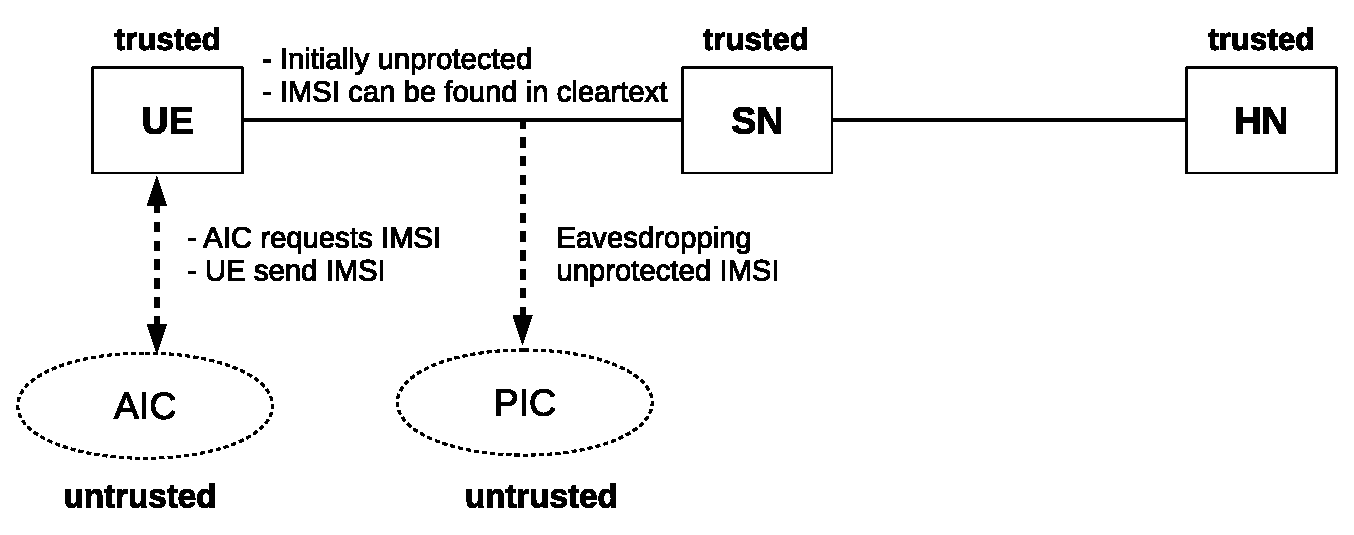
\includegraphics[height= 4cm]{security_architecture_abstraction.eps}
% figure caption is below the figure
\caption{High-level security architecture}
\label{fig:security_architecture_abstraction}       % Give a unique label
\end{center}
\end{figure} 

\subsection{Current Solution Approach and its Weakness}
One approach of protecting IMSI privacy is to use a temporary identifier instead of the actual IMSI and keep changing the temporary identifier frequently. Note that the temporary identifier has to be assigned confidentially. Different entities of the network may assign different temporary identifiers to the UE. 

In the LTE network, the temporary identifier assigned by an SN is called globally unique temporary identity (GUTI) and the HN does not assign any temporary identifier to the UE. However, during the initial attachment of a UE to the SN, the UE has neither a GUTI nor a security context with the SN that can assign it with a GUTI. Besides, GUTI can be lost by either one or both of the UE and the SN. This would force the UE to reveal its IMSI to the SN to keep itself from permanently locked out of the network.

This problem gives an opportunity to an AIC who impersonates a legitimate SN and forces the UE to run the initial attachment protocol. This also gives an opportunity to a PIC to eavesdrop the IMSI sent in cleartext. Solutions \cite{pseudonym_valtteri_philip,pseudonym_ericsson,CCS15,SSR15} have been proposed by using temporary IMSI known as pseudonym. While these solutions solve the cases of lost and unsynchronised GUTI, they still have the problem of lost or unsynchronised pseudonyms. Public-key technologies have also been considered as potential approach to solve this problem.

\section{Discussion on Different Proposed Solutions}\label{sec:solutions} 
\label{sec:existing_solutions}
Before delving into different proposed those solutions, let us introduce some notation. 
\begin{enumerate}
\item $hnid,snid=MCC||MNC$ identifies the HN and SN respectively
\item $e_A,d_A$ is the public and private key of entity $A$ respectively
\item $\mathcal{X}_{A,B}(e_A,e_B)$ is the certificate of the public key $e_A$ of $A$. The certificate can be verified by anyone who considers $B$ as a root CA using the public key $e_B$. The certificate is a guarantee from B that the public key $e_A$ is owned by $A$ .
\item $E,D$ are encryption and decryption functions so that $D(E(M,K),K) = M$.
\item $S(M,K)$ is the signature of message $M$ signed by the key $K$
\end{enumerate}

\subsection{Solution Based on Pseudonyms:}
\label{sec:pseudonyms}
Pseudonym based solutions have been proposed in \cite{pseudonym_ericsson,pseudonym_valtteri_philip,CCS15,SSR15}. In this kind of solutions, temporary identifiers called pseudonyms are assigned to a UE. Next time when the UE tries to identify itself to an SN, it uses a pseudonym instead of IMSI. Periodically, whenever there is an opportunity, the HN sends a new pseudonym to the UE with confidentiality and integrity protection. One such opportunity could be when the HN sends the authentication vector to an SN.

\subsection{Solution Based on Certificate Based Public-key Cryptography} 
\label{sub_sec:solution_certificate}
Use of certificate based public-key encryption to conceal long-term identity has been suggested in 3GPP TR 33.821 \cite{TR33821}. To use certificate based public-key cryptography, we need to figure out who are the root CAs and who else can be a CA, who own a public key, how a certificate can be revoked, and how the UE can be re-provisioned with a new root certificate if needed. Different solutions can be devised based on the choice of root CAs and other CAs. We provide a high-level description for few variants of certificate based solution.

\subsubsection{Variant 1:}
It uses a global root of trust. There is a global entity trusted by everyone. Using this trusted global entity, a chain of trust can be established. The SN presents the certificate to a UE trying to attach. The UE verifies the certificate. If the verification result is positive, the UE encrypts its IMSI using the public key of the SN and sends to the SN. 

\subsubsection{Variant 2:}
In this variant the HN of a subscriber is the root CA. The HN generates a public-private key pair and generates a certificate of the public key signed by the HN itself. A UE is provisioned with this self signed certificate. An SN interested to serve a UE obtains a certificate $\mathcal{X}_{snid,hnid} (e_{snid},e_{hnid})$. The UE sends $hnid,e_{hnid}$ to the SN. The SN looks up for the certificate $\mathcal{X}_{snid,hnid} (e_{snid},e_{hnid})$. In case it exists at the disposal of the SN, the SN sends it to the UE. The UE verifies the certificate. If the certificate is verified as valid, then the UE sends the IMSI to the SN encrypted by the public key $e_{snid}$ of the SN.

\subsubsection{Variant 3:}
In this variant, there is no other CA than the root CA. Hence the chain of certificates is very short. Only an HN can be a CA. The certificates of all the SNs a UE might visit are pre-provisioned to the UE by the HN. When a UE attempts to attach to an SN, the UE encrypts the IMSI with the public key of the SN which is already provisioned to the UE. If the public key of an SN is revoked, the HN has to provision the revocation to the UE.


\subsection{Solution Based on Root-key based Encryption} 
\label{sub_sec:solution_root-key}
We use only one pair of public-private key pair in this approach. Such a technique has been proposed in 3GPP TR 33.899 in solution \#7.3. This key pair is owned by the HN and we call it to be the root-key. The HN provisions the public key to all its UEs.  Instead of sending the IMSI, the UE encrypts the IMSI with the public root key and sends the result to the SN along with the $hnid$. The SN sends the encrypted IMSI to the HN. The HN decrypts the IMSI and sends the IMSI back to the SN along with an authentication vector (AV).

\subsection{Solution Based on IBE}
In the next section we discuss the basic principles of IBE and present a solution of the identity privacy using IBE. 


\section{Details of the IBE Based Solution} 
\label{sec:solutions_based_on_IBE}
\subsection{How IBE works}
The idea of IBE was proposed by Adi Shamir in 1984 \cite{IBE_shamir}. For last two decades, there have been significant research effort in finding new IBE schemes. For example, Dan Boneh and Matthew Franklin published a fully functional IBE scheme in 2003 \cite{IBE_boneh_franklin} and Clifford Cocks presented an implementation in 2001 \cite{IBE_clifford}. There are plenty of other schemes. There are also a range of international standards e.g., ISO/IEC 11770-3, ISO/IEC 14888-2, ISO/IEC 14888-3, IEEE P1363.3. In this paper we do not investigate into these schemes and standards. Rather we investigate how a general IBE scheme can be used to solve the identity privacy problem in the cellular networks. We believe an appropriate standardized IBE scheme can be chosen later based on other niche practical requirements of the networks. However, we present a very simple description of how IBE works so that the readers can follow our proposed solution easily. 

The fundamental difference between IBE and certificate based public key encryption is how the keys are generated and managed. In IBE, the public key of a receiver is computed as a function of the identity of the receiver in conjunction with the public key of a trusted third party. Similarly, the private key of a receiver is computed as a function of the identity of the receiver in conjunction with the private key of the trusted third party. Since the private key of the trusted third party is known only by the trusted third party, no one else than the trusted third party can compute the private key of a receiver. The trusted third party will provision a receiver with the private key through some other secured channel. Consequently, a sender does not need to authenticate the public key of a receiver. In IBE, the authenticity of the public key of a receiver is guaranteed by the trusted third party. Usually in IBE, the trusted third party is known as the private key generator (PKG). Figure \ref{fig:how_IBE_works} shows the mechanism.


\begin{figure}
\begin{center}
% Use the relevant command to insert your figure file.
% For example, with the graphicx package use
  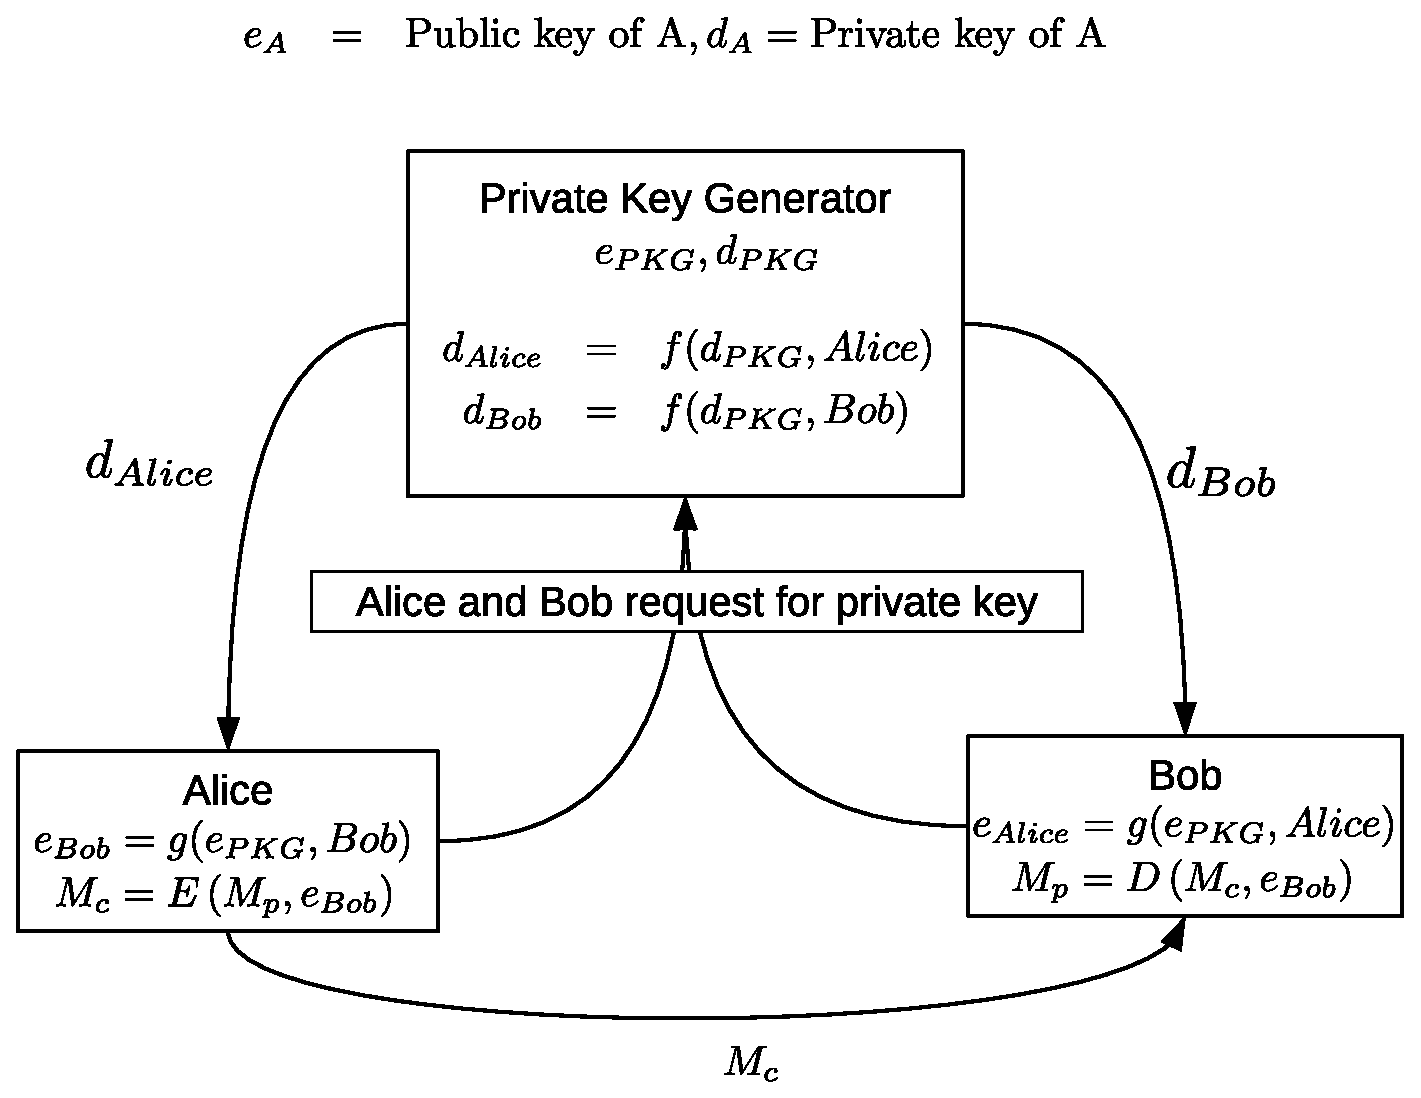
\includegraphics[height=7cm]{how_IBE_works.eps}
% figure caption is below the figure
\caption{How IBE Works}
\label{fig:how_IBE_works}       % Give a unique label
\end{center}
\end{figure}

Relevant constraints of an IBE scheme:
\begin{enumerate}
 \item The private key of the receiver has to be provisioned to the receiver by the PKG.
 \item It is impossible to revoke the public key in IBE unless the identity itself is revoked.
 \item Since a PKG knows the private keys of all the receivers, a PKG can decrypt any message sent by any sender to any receiver. This implies that there must be a very high level of trust in the PKG.
\end{enumerate}

\subsection{Existing Proposals of Using IBE in Cellular Network}
Jo, Paik and Lee proposed a privacy-preserving authentication protocol in wireless mobile network in 2014 \cite{IEE_transactions_mobile_computing_2014} based on a pseudo-identity-based signcryption scheme. In this protocol the authors do not discuss how the public key of the SNs can be revoked. This protocol is not designed for the 3GPP defined cellular networks specifically but for any wireless mobile network. Naturally there are 3GPP specific requirements that the protocol does not address at all, e.g., the identity of a user is kept secret even from the SN which is not allowed in 3GPP networks. In the rest of the paper we will refer this protocol as JPL protocol.

Geir M. K{\o}ien proposed a privacy enhanced mutual authentication protocol in LTE in 2013 \cite{koienibe} based on IBE. The author named the proposed protocol as PEMMA. In PEMMA, the HN is the PKG and the SNs own public-private key pairs. In PEMMA the UE encrypts the IMSI using the public key of the SN before sending the IMSI. Consequently PEMMA can conceal the IMSI. However, the author designed PEMMA so that it requires all the three parties (UE,SN and HN) to be online during the authentication. Consequently PEMMA can not support the situation where the SN want to use a pre-fetched AV. Also, in PEMMA, the authentication delay would most likely be dominated by the physical distance between the SN and the HN when they are in different continents. It would be desirable to have an authentication protocol that can run even without contacting the HN when the HN is far from the SN. Besides, PEMMA requires an SN to agree with all the HNs on the same expiry date for its public key. It is not likely that a particular SN will be trusted to the same extent by all the HNs.

RFC 6508 \cite{RFC6508} presents an algorithm SAKKE for establishment of a secret shared value. Applications of SAKKE may include a date-time component in their identity to ensure that identities and hence the corresponding private-keys are only valid for a fixed period of time. Solution \#7.11 in 3GPP TR 33.899 \cite{TR33899} uses IBE to protect the long-term identity according to RFC 6508. However, the solution does not address the issue of revocation of the identity based public-keys. RFC 6507 \cite{RFC6507} describes a certificate-less signature scheme based on IBE. In this scheme a string called public validation token (PVT) randomly chosen by the PKG is assigned to an identity. Both the public and private key of a receiver are computed using the PVT along with the receiver's identity. So, the public key associated with an identity can be revoked by revoking the PVT. Solution \#2.14 in 3GPP TR 33.899 presents an authentication framework based on the signature scheme of RFC 6507 and the authentication protocol EAP-TLS. This solution uses the PVT to revoke the public key associated with an identity. However, in this solution it is not clear how a UE can check if the public key of an SN has been revoked or not.

\subsection{Our Proposed Solution}
Next we present a protocol that serves the purposes of both privacy protected identification of UE and mutual authentication between UE and SN. This mutual authentication does not require a contact with the HN each time the protocol is run between a UE and an SN. Hence a fast mutual authentication is achieved when SN and HN are located far from each other. We call this protocol as privacy enhanced fast mutual authentication (PEFMA).


In PEFMA, the HN is the PKG. PEFMA does not use PVT but instead use an expiry time (ET). This expiry time can act as the PVT. HN computes private keys of all of its users using their IMSIs and suitably chosen ETs. These private keys are provisioned to the UEs using a secured channel. The SNs which have a roaming agreements with the HN are also provisioned with their respective private keys by the HN. Before the expiration of the ET, a UE or an SN may request for a new private key to the HN. The HN would choose a new ET, compute the private key and send the new private key to the UE or to the SN in a secure channel. A UE may request for a new private key if the UE believes that the private key has been compromised.


PEFMA protocol may run when a UE is asked to reveal its IMSI. If a UE identifies itself using a temporary identity and the SN can not recognize the temporary identity, the SN asks the UE to reveal the IMSI. If the temporary identity used by the user is recognized by the SN then the SN may run the PEFMA protocol if there is no appropriate pre-fetched AV available in the SN and the HN is far from the SN. If the HN is near, the SN will fetch an AV and run the traditional UMTS or LTE AKA. If there is already an appropriate pre-fetched AV available, the SN runs the appropriate AKA protocol. Note than an UMTS/LTE AKA will follow at some point after PEFMA is successfully run. PEFMA is run to ensure fast authentication without contacting the HN. The following AKA ensures that the user is not impersonating another legitimate user by stealing the private key. The following AKA may run at a point of time chosen by the SN. Figure \ref{fig:when_pefma_runs} shows pictorially when PEFMA is run.


If the public key of a user needs to be revoked, the expiry time along with the identity of the user is added to the revocation list. If the user requires a new public key (e.g., the old one is compromised), the PKG uses another expiry time to compute the private key of the user. The newly computed private key is then provisioned to the identity along with the the new expiry time. When the expiry time comes, all the public keys computed using the expiry time are automatically revoked. So, the revocation list does not need to include revocations whose expiry time is in the past. 


\begin{figure}
\begin{center}
% Use the relevant command to insert your figure file.
% For example, with the graphicx package use
  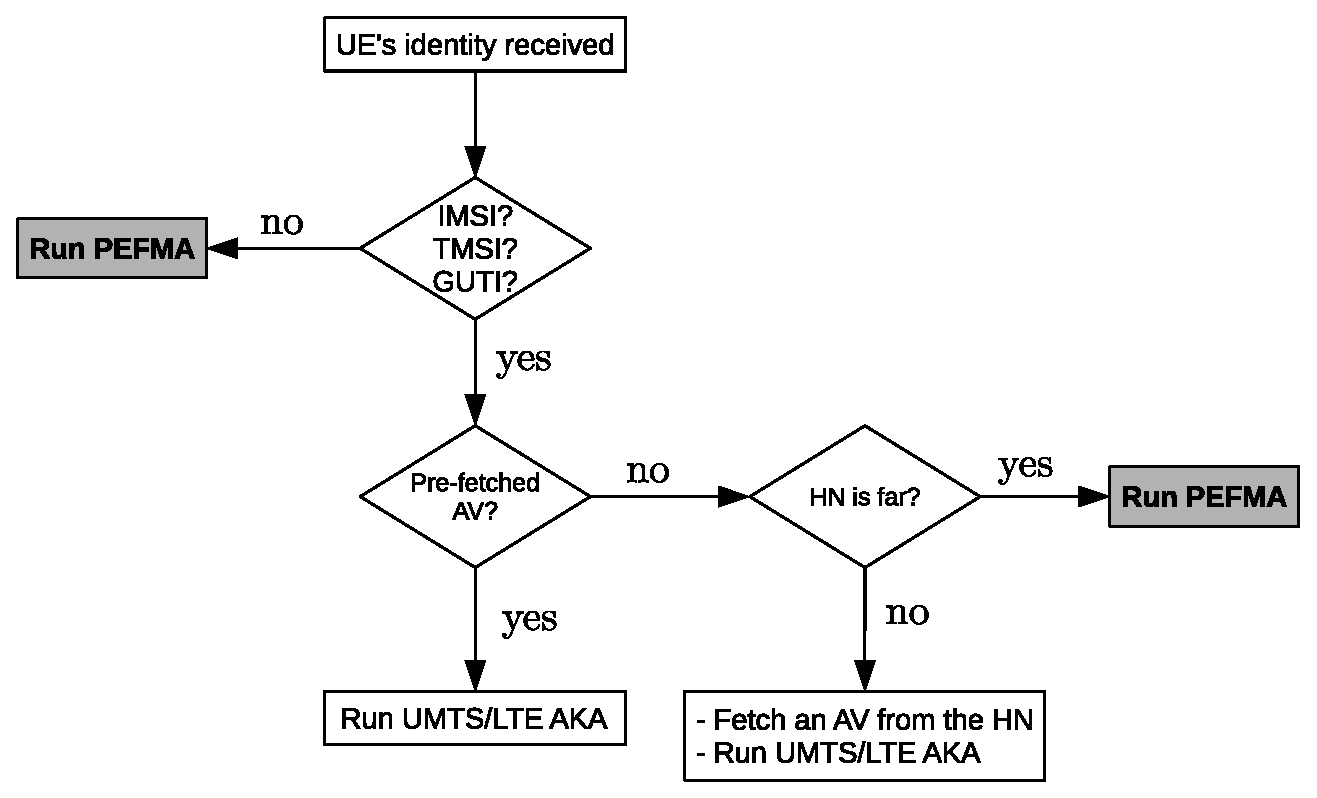
\includegraphics[height=9cm]{when_to_run_PEFMA.eps}
% figure caption is below the figure
\caption{When PEFMA Runs}
\label{fig:when_pefma_runs}       % Give a unique label
\end{center}
\end{figure}


\begin{figure}
\begin{center}
% Use the relevant command to insert your figure file.
% For example, with the graphicx package use
  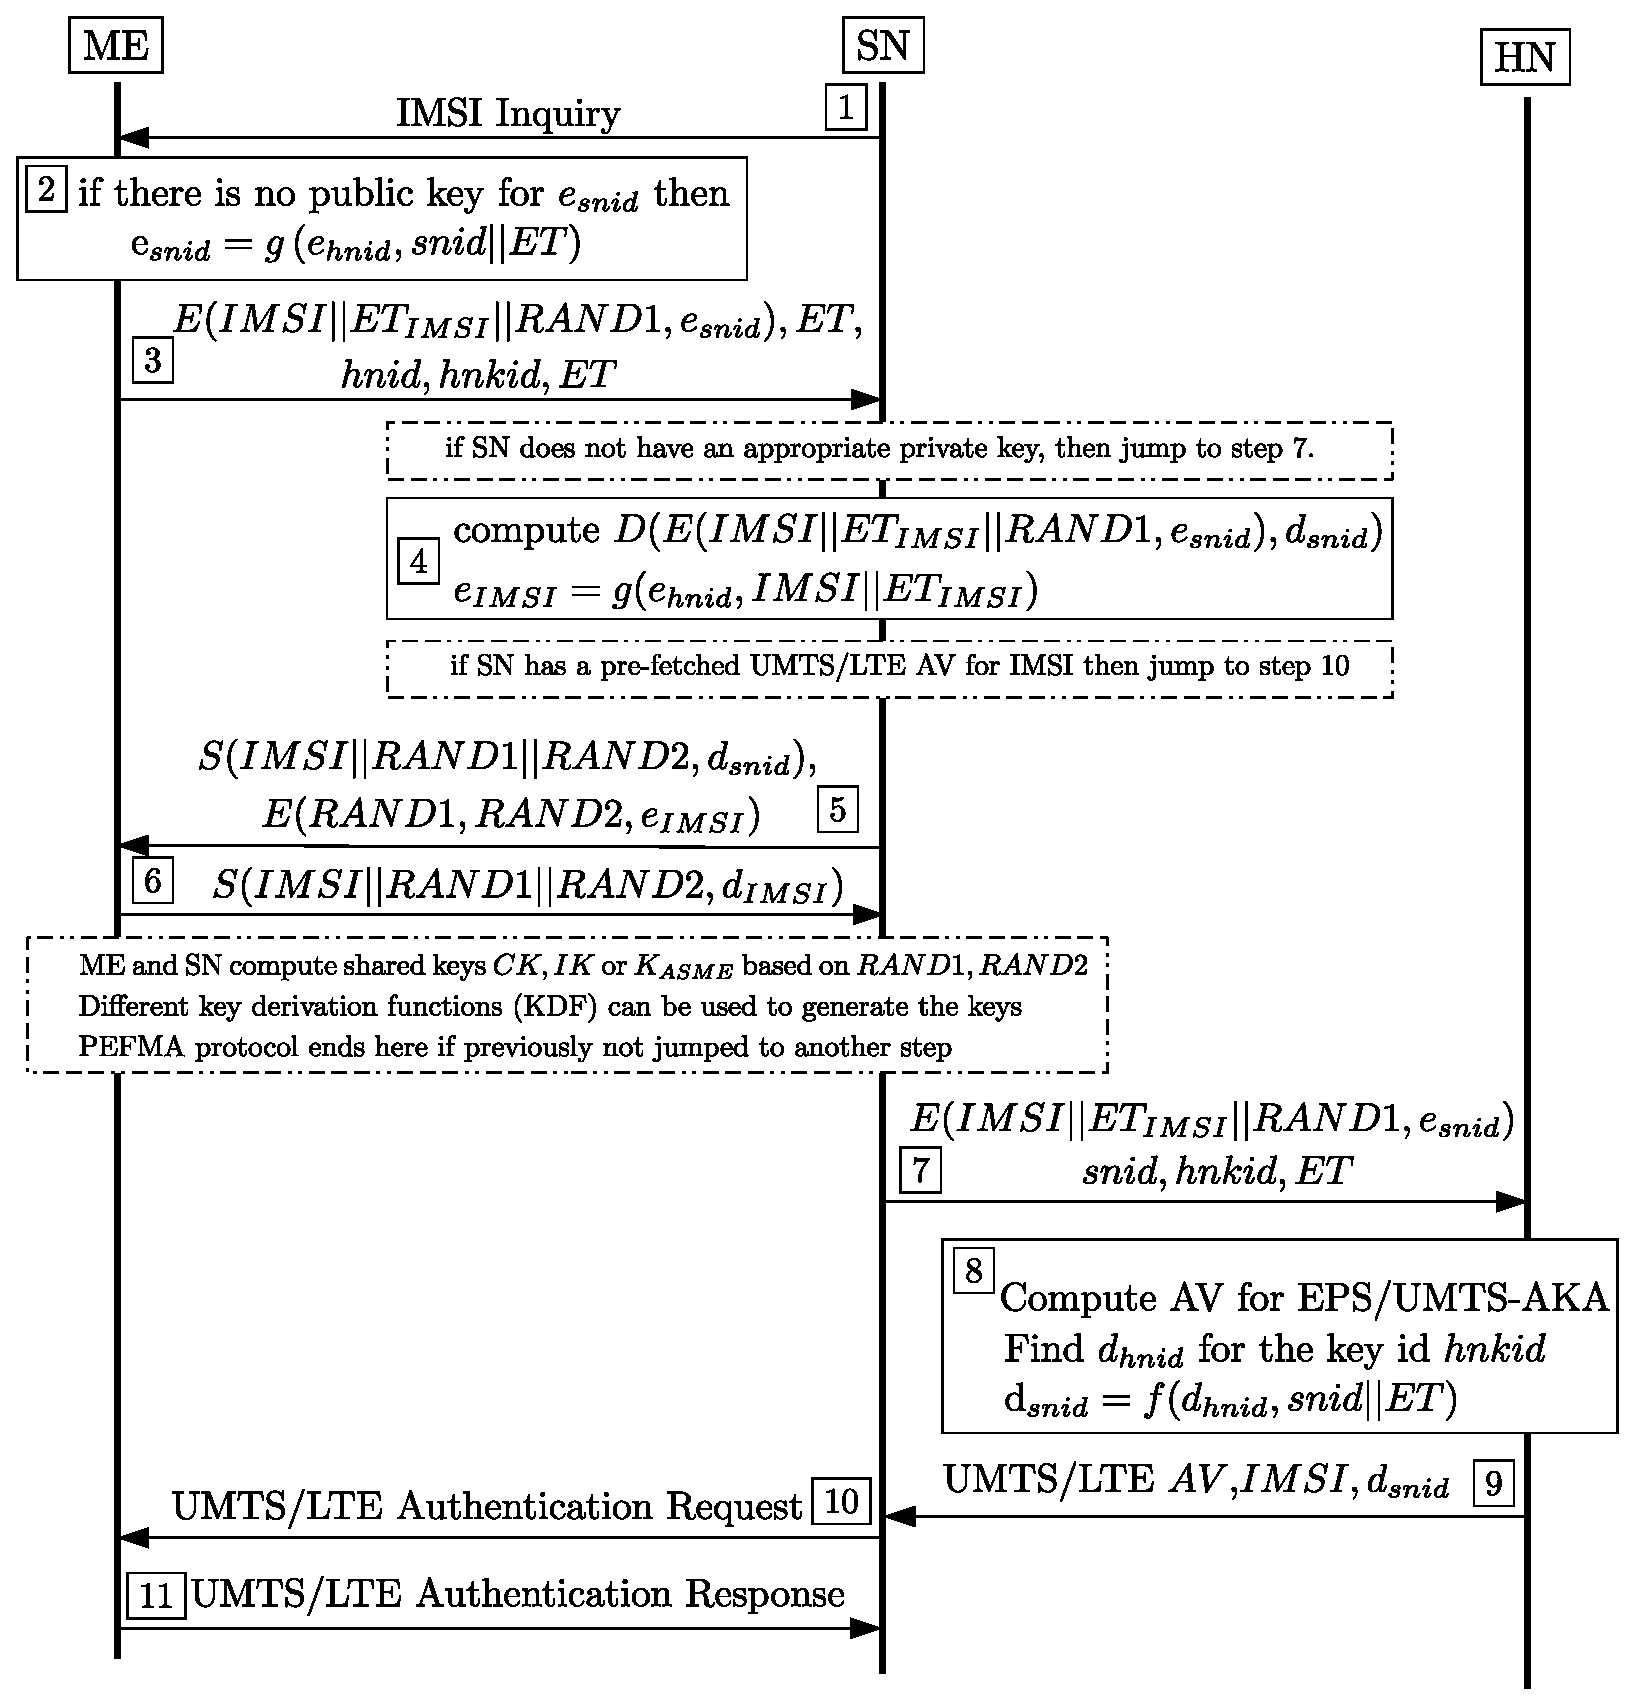
\includegraphics[height=12cm]{PEFMA.eps}
% figure caption is below the figure
\caption{PEFMA}
\label{fig:PEFMA}       % Give a unique label
\end{center}
\end{figure}



\subsubsection{PEFMA}
The UE's HN acts as the PKG. The solution is pictorially presented in Figure \ref{fig:PEFMA}. The description follows:

\begin{itemize}
\item[1:] The SN makes an IMSI Inquiry to the UE. 
\item[2:] The UE computes $e_{snid} = g\left(e_{hnid},snid||ET \right)$
\item[3:] The UE sends $E(IMSI||ET_{IMSI}||RAND1,e_{snid}),hnid,hnkid,ET$ to the SN. Here $ET_{IMSI}$ is the expiry time of the public-private key pair of the UE. $RAND1$ is a random challenge chosen by the UE using a secure random number generator function. $hnkid$ is the key ID of the HN that is used by the UE to compute $e_{snid}$
\item[4.0:] The SN looks for a private key $d_{snid}$ that is compatible with $hnkid$ and $ET$. If not found, it jumps to step $7$, otherwise continues from step $4$.
\item[4.1:] The SN extract $IMSI,ET_{IMSI}$ and $RAND1$ received in step $3$. The SN also computes the public key of the UE $e_{IMSI}$ using the public key of the HN identified by $hnkid$ as $e_{IMSI} = g(e_{hnid},IMSI||ET_{IMSI})$.
\item[4.2:] If the SN has a pre-fetched UMTS/LTE AV for IMSI then jump to step $10$.
\item[5:] The SN chooses a random challenge $RAND2$ using a secure random number generator function. The SN encrypts both $RAND1$ and $RAND2$ using the public key of the UE computed in step $4.1$. The SN also signs the message $IMSI||RAND1||RAND2$ using its private key $d_{snid}$ and send the signature to the UE so that the UE can verify it using the SN's public key. 
\item[6:] The UE extracts $RAND1$ and $RAND2$ using its private key $d_{IMSI}$. It verifies the signature received in step $5$ using the public key $e_{snid}$. If the verification is successful, the UE signs the message $IMSI||RAND1||RAND2$ using its private key $d_{IMSI}$. The SN verifies the signature using the public key $e_{snid}$. If this verification is successful then authentication is completed and both the UE and SN are mutually authenticated to each other. Based on $RAND1$ and $RAND2$ they can create shared secrets $CK,IK$ or $K_{ASME}$ as required using key derivation functions.

\item[7:] If the SN does not have the appropriate private key to decrypt the message it received in step $3$, it forwards the received message to the HN. The SN might not have the appropriate private key because the UE is using an $ET$ for which the SN has not been provisioned with a private key by the HN. Another reason could be that the UE and SN are having different public keys $e_{hnid}$ identified by different $hnkid$. The reason for having different public keys $e_{hnid}$ could be that the HN has switched to a new public-private key pair while either the UE or the SN is not yet aware of the change.
\item[8:] Given $snid,hnkid$ and $ET$, the HN can compute the appropriate $d_{snid}$. The HN then extracts $IMSI,ET_{IMSI}$ and $RAND1$ using $d_{snid}$. The HN then prepares an appropriate (UMTS/LTE) $AV$ for the received $IMSI$.
\item[9:] The HN forwards the $IMSI,AV$ and the private key $d_{snid}$ to the SN. The SN stores the $d_{snid}$ mapped with the respective $hnkid$ and $ET$ so that next time a UE uses the same $hnkid,ET$, the SN would not need to contact the HN.
\item[10:] The SN has an $AV$ and based on the $AV$ it sends an UMTS or an LTE authentication request to the UE.
\item[11:] The UE sends the appropriate UMTS or LTE authentication response to the SN.
\end{itemize}


\subsection{Provisioning}
The UEs and the SNs need to be provisioned with their respective private keys and the HN's public key. Keys will be expired and new keys will be needed to be provisioned. Keys might be compromised and be needed to be revoked (key revocation is discussed in next section). Once a key is revoked, a new key is needed to be provisioned to the appropriate entities (either to UE or SN, or both).

An SN is provisioned with the public key $d_{hnid}$ of an HN and with a key ID $hnkid$ first time when a roaming contract is signed between the SN and the HN. When the public key of the HN expires or the private key be compromised (an extremely rare event), the HN chooses a new public-private key pair. This new public key along with the new $hnkid$ is provisioned by the HN to all the SNs who have a roaming contract with the HN.There is already a secure channel between a HN and an SN, hence the keys can be provisioned with both confidentiality and integrity protection. The HN also provisions all the UEs who are in home and have a valid security context with the new public key and the respective $hnkid$ via the control plane. Messages in the control plane are both confidentiality and integrity protected.

The SN does not request for a new private key even if the SN believes that its private key has been compromised. Because there is no way to inform the UE about it and consequently getting a new private key does not not help in anyway. When the expiry time of the compromised private key comes, the key is automatically expired. Hence, the expiry time of the public-private key pairs of SNs' is recommended to be near in the future.

We design our solution so that no change is required in the USIM. This enables the legacy USIMs to work with our solution without any change. This means, the public key of the HN and the private key of the UE have to be provisioned to the ME. When a USIM is inserted into an ME, the ME has no idea about the respective HN's public key and the UE's private key. So, for the very first time after a USIM is inserted in an ME, the UE identifies itself with the IMSI. This is not a problem because this IMSI will not be used anymore while the USIM is inside the same ME. Once authentication is successful between the SN and the UE, there is a security context available. If the UE is not roaming then the ME requests for key provisioning via the control plane and the SN (which is also the HN) sends back the public key of the HN along with the key ID and the private key of the UE along with the $ET_{IMSI}$ also via the control plane. This message is both confidentiality and integrity protected since it is exchanged via the control plane. Note that the UE can not be provisioned with the keys when it is roaming.

If a UE believes that its private key has been compromised, and if the UE is not roaming then it requests for new keys to the HN via the SN. HN revokes the current key of the UE, chooses a new $ET_{IMSI}$, compute the new private key and send the new private key along with the chosen $ET_{IMSI}$. The SN forwards the same to the UE with both confidentiality and integrity protection via the control plane.

The UEs also have to be provisioned with the list of all the trusted SNs and if they are able to run PEFMA. Such provisioning can be done similarly as the keys are provisioned via the conrol plane when there is a security context. If a UE is offered service by an SN who is not in the trusted list and also does not have PEFMA ability, the UE rejects the offer. If the SN is in the trusted list but does not have PEFMA ability, the UE may accept the offer and reveal the IMSI for authentication.

\subsubsection{Key Revocation}
The $ET$ used to generate the public key $d_{snid}$ is quite near in the future, e.g., the day end. So, if the public key needs to be revoked, it would automatically be revoked when the expiration time comes. In this way, a compromised SN would be able mount an attack only for a short period of time. However, the SN would need to get new $d_{snid}$ from the HN before the old $d_{snid}$ expires. 

When the public key of a UE is revoked, the IMSI and relevant $ET$ is stored in a revocation list in the HN.  An SN serving UEs of an HN has a copy of the list. The SN also periodically checks with the HN if there is any new revocations. Before computing the public key of the UE, the SN checks the revocation list. If it is revoked, the SN discards the message received from the UE and the authentication fails. 

All the entries with expiry time older than current date-time can be removed from the revocation list, hence the revocation list will not grow to a very large size. This frequent private key exchange and refreshing the revocation list would create a bit increased traffic between an SN and HN. On the other hand, this increased traffic is not in the air interface but in the back haul network, which apparently is not very critical. 

\subsection{Discussion and Evaluation}
\subsubsection{Identity Privacy}
A PIC can learn the IMSI of a user during the first time the UE identifies itself after the USIM is inserted into an ME. Moving USIM from one ME to another is a very rare event and the PIC would have a very tiny chance in catching an IMSI. However, a PIC learn the $hndi$ of a subscriber who identifies itself using the encrypted IMSI.

All a PIC can do, an AIC is also able to do. However, an AIC can still impersonate a legitimate SN and present itself as not PEFMA enabled. The UEs will be provisioned by the HN with the list of the PEFMA enabled SNs it might visit. An PEFMA enabled UE will never reveal its IMSI to an SN which is in the trusted list and marked as PEFMA enabled. Over the time as more and more SNs become PEFMA enabled, the success rate of an AIC in catching an IMSI decreases.


\subsubsection{Impact of compromised/lost private keys}
If the UE's private key is compromised, the attacker who has the compromised key can learn the IMSI and can impersonate the user by running PEFMA protocol. The attacker can do this until the compromised key is revoked. However, even before the revocation, when UMTS/LTE AKA is run, the attacker would not be able to pass through and consequently be denied any service. This means, using a compromised private key of a user, an attacker can impersonate the user only until the compromised key is revoked and only until the UMTS/LTE AKA is run. If the private kye of the user is lost but not compromised, the user can still identify itself using encrypted IMSI but can not perform PEFMA which implies the user can not participate in the fast authentication without involving the HN. Nevertheless, UE's compromised/lost private key can not keep it from authenticating itself to the SN hence the user still remain connected with all the services. When the user comes to the HN, a new private key can be provisioned to the UE by the HN.

If an SN's private key is compromised, an attacker who knows the compromised key can impersonate the compromised SN to a UE, can run PEFMA and consequently can breach the identity privacy, data confidentiality and integrity. However, once the key expiry time comes the compromised key is automatically revoked and the attacker can not attack anymore thereafter. However, compromisation of SN's private key is an extremely rare event. Even if it happens, the attacker can not keep attacking for long since the expiration time of SN's private-public key pair is near in the future. If SN's private key is lost but not compromised, the SN can not identify any user of the respective HN and hence can not provide any service until the SN get private key from the HN. However, losing the private key is also an extremely rare event. Even if it happens, the SN knows it immediately a user from the respective HN visits. This means, the SN can be quickly re-provisioned with the private keys by the HN.

If the HN's private key is compromised, the attacker who has the compromised key can impersonate itself as any SN who has a roaming contract with the HN. The attacker can then run PEFMA with any subscriber of the HN and consequently can breach identity privacy, data confidentiality and integrity. The attacker can also impersonate as a subscriber with an IMSI which belongs to the HN and consequently can avail services. However, compromisation of HN's private key is an extremely rate event. Even if it happens, once the compromisation is detected, the HN can generate a new public-private key pair and re-provision all the SNs and UEs with a new public key. 


If the HN's public key is lost, no UE and SN can be provisioned with private keys any more. This implies that after the expiration of the private key of an SN, the SN would not be able to identify a user who tries to identify itself using the encrypted IMSI. The HN chooses a new public private key pairs and provisions the new public key to all the SNs and all the UEs who are already assigned a TMSI or GUIT and currently not roaming. However, all the UEs who are roaming or are not assigned a TMSI or GUTI remains out of the network until it manually get the new public key of the HN.

\subsubsection{Effectiveness and Efficiency}
PEFMA is effective when both the UE and the SN are PEFMA enabled. However, when an SN is not PEFMA enabled and in the trusted list, an attacker can mount an active IMSI catching attack. Nevertheless, over the time more and more SNs become PEFMA enabled and IMSI privacy enhances. It is better than some other approaches that need a hard cut off date for implementing the solution. PEFMA is also transparent to the USIM.  
Patching the legacy MEs will be the challenge. On the other hand, when the 5G MEs can be patched with PEFMA ability before making them available in the market. Thus, a user switching to a 5G enabled ME avail PEFMA ability even for UMTS or LTE network. 

Unlike PEMMA \cite{koienibe}, PEFMA does not require to standardize the ET (expiry time of the key of an SN) so that all the HN assigns the same ET to a particular SN. Instead, in PEFMA, all the UEs of a particular HN uses the same ET when they go roaming. This means an SN will need a private key associated with the HN and the ET used by the UEs of the HN. In this way, ET needs to be standardized only within a single HN, not across all the HNs.

PEFMA will introduce some extra signalling and computational overhead between UE and SN due to public key encryption and introduction of new message flows. However, PEFMA will run very infrequently and hence the additional signaling overhead may not be much of a problem. Private keys of SNs would need to be frequently provisioned by the HN. Generating private keys frequently would add some additional computational load on HSS. However, HSS is a very powerful server and should be able to serve the extra load.

One usability issue is that, a user can not move its USIM from one ME to another while roaming. If does so, the new ME can not be provisioned with the HN's public key and the users private key and hence the users IMSI privacy will become vulnerable to an AIC until the user go back to the HN.


 %\begin{sidewaystable}
\begin{table}
\begin{tiny}
 \begin{center}
\caption{Comparative evaluation of the solutions}
\begin{tabular}[t]{|l|c|c|c|c|c|c|c|c|}
\hline
\multicolumn{1}{|c|}{} & \multicolumn{1}{|c|}{} & \multicolumn{7}{|c|}{\textbf{Public-key based Solutions}}\\
\cline{3-9}
\multicolumn{1}{|c|}{\textbf{Criteria}} & \multicolumn{1}{|c|}{\textbf{Pseudonym}} & \multicolumn{3}{|c|}{\textbf{Certificate based}} & \multicolumn{1}{|c|}{\textbf{Root-key}} & \multicolumn{3}{|c|}{\textbf{IBE based}}\\
\cline{3-5} \cline{7-9}
\textbf{} &  & \textbf{V1} & \textbf{V2} & \textbf{V3} & \textbf{} & \textbf{JPL} & \textbf{PEMMA} & \textbf{PEFMA}\\
\hline \hline
Immunity to AIC & + & + & + & + & + & + & + & + \\ \hline
Concealing $hnid$ & - & + & - & - & - & + & - & - \\ \hline
Lawful interception & + & + & + & + & - & - & + & + \\ \hline
Mutual Authentication & - & + & + & + & - & + & - & + \\ \hline
Signaling overhead & + + & - & - & - & + & + & + & + \\ \hline
Computational overhead & + & - & - & - & + & + & + & + \\ \hline
Latency while roaming & - & - & -  & - & - & + & - & + \\ \hline
Latency while at home & + + & - & -  & - & + & + & + & + \\ \hline
PKI effort & + + &  - & + & + & + & + & + & + \\ \hline
Key revocation & ++ & - & - & - & + & - & - & - \\ \hline
Provisioning effort & + & + & + & - & + & + & + & + \\ \hline
Using existing gear & + & - & + & + & + & - & + & + \\ \hline
Maturity  & - & + & + & - & + & - & - & - \\ \hline
\end{tabular}
\label{table:comparison}
\end{center}
\end{tiny}
\end{table}
%\end{sidewaystable}




\section{Qualitative Comparison of Different Solutions}
\label{sec:evaluation}
In this paper we have discussed two different categories of solutions: pseudonym based and public-key based. Different solutions \cite{pseudonym_valtteri_philip,pseudonym_ericsson,CCS15,SSR15} have been and more could be devised based on pseudonyms. All these solutions would require the UE and the HN to synchronize their pseudonym states between a UE and the HN.

We have categorized the different public-key technologies into three categories: certificate based, root-key based and identity based. None of them require to maintain synchronization of states between a UE and the HN. But these solutions have some downsides. They need comparatively heavier computational resources, and the ciphertext are longer which affect the latency. All these Solutions require a mechanism of key revocation.

In certificate based solutions there is a need of a global PKI. However, in some variants of certificate based solutions, the effort to manage a PKI can be reduced significantly. Certificate based solutions require an extra round trip between the UE and SN to exchange and verify the certificate. In a variant of a certificate based solution, this extra round trip could be removed at the expense of provisioning the certificate of an SN to a UE before the UE goes roaming to the SN. All the certificate based solutions have the requirement of exchanging certificates and verifying them. This creates signaling and computational overhead which consequently affect the latency. 

The root-key based solution does not require any extra round trips or certificates, hence it has better signaling and computational overhead compared to certificate based. However, it still suffers from the increased latency in a roaming situation because every authentication needs to travel all the way to the HN. This is because no one else except the HN can decrypt the message sent by the UE. The solution creates also computational pressure in the HN. 

In the category of identity based solutions, the JPL scheme was not designed specifically for the 3GPP defined networks and hence does not support an important 3GPP requirement: LI. It also does not support the revocation of the private keys of the SNs. PEMMA needs all the three parties (UE,SN and HN) to be online which implies higher latency. PEMMA also requires high standardization effort to revoke the public private key pairs of the SNs.

Our novel solution based on IBE that we call PEFMA, can both accomplish the identification and mutual authentication. The solution does not need to maintain synchronized states between a UE and the HN. The solution does not require a global PKI and does not need certificates. Unlike the root-key based approach, our solution does not need to involve HN each time authentication is needed. It requires standardization effort only within a single HN. The solution can co-exist with the existing protocols and does not need a hard cut off date for implementation. The aforementioned argument makes the IBE based solution a potential candidate to solve the problem in question. In Table \ref{table:comparison}, we present a comparison among the different solutions based on different criteria.

Apparently pseudonym based solution is very good in most of the criteria. One downside of pseudonym based approach is, if the pseudonym is unsynchronized between UE and HN, the user has to visit the HN physically and get back to synchronized state by giving the IMSI in a trusted environment. The need of visiting the HN physically might make the pseudonym based solution a little clumsy. Variant 1 of certificate based approach is good in preventing AIC and also conceals $hnid$. But this is bad in many other important criteria because of exchanging and verifying certificates. Considering the concealment of $hnid$ with a bit less priority, the CertV1 is outperformed by both root-key based and IBE based solution. CertV2 and CertV3 can not even conceal $hnid$. So, the extra overhead of using Certv2 and CertV3 is not worth comparing to root-key, PEMMA or PEFMA. When comparing PEMMA, PEFMA and root-key, all of them are almost similar except that PEMMA and PEFMA provide mutual authentication. However, Cert1V can also be extended to a mutual authentication protocol. 

If concealing $hnid$ is essential, then the only applicable solution is Certv1, the certificate based solution with global root of trust. If concealment of $hnid$ can be compromised, then the choice  of the solution depends on the requirement of mutual authentication. If mutual authentication of UE and SN without involving HN is considered important and useful then PEFMA is the winner. Otherwise, root-key based solution is just enough.


\section{Conclusion}
\label{sec:conclusion}In this paper we have discussed different known approaches to conceal the IMSI. The solutions  are based on pseudonyms and public-key encryption. We have proposed a novel solution based on identity based encryption that serves the purposes of both identification and mutual authentication. We have used expiry time as part of the identity of the entities in the system. We have presented a qualitative comparison between different  solutions. We argue that identity based encryption is a competitive solution when concealing the home network identity is not necessary and mutual authentication in between a user equipment and a serving network is useful without connecting with the home network. The comparison is based on qualitative analysis based on known facts of public-key cryptography.



%\subsubsection{Acknowledgement.}
%\label{sec:acknowledgement}

%\appendix

%And this is my Appendix.

%\subsection*{Appendix Subsection}

%Some text.

\nocite{*} % add all entries from sample.bib


%\bibliographystyle{plain}
%\bibliography{mybib}{}

\begin{thebibliography}{10}

\bibitem{RFC6507}
{RFC} 6507 {C}ategory: {I}nformational.
\newblock \url{https://tools.ietf.org/html/rfc6507}.

\bibitem{RFC6508}
{RFC} 6508 {C}ategory: {I}nformational.
\newblock \url{https://tools.ietf.org/html/rfc6508}.

\bibitem{TR21905}
3GPP.
\newblock {3GPP TR} 21.905.
\newblock
  \url{https://portal.3gpp.org/desktopmodules/Specifications/SpecificationDetails.aspx?specificationId=558}.

\bibitem{TS23003}
3GPP.
\newblock {3GPP TS} 23.003.
\newblock
  \url{https://portal.3gpp.org/desktopmodules/Specifications/SpecificationDetails.aspx?specificationId=729}.

\bibitem{TS33106}
3GPP.
\newblock {3GPP TS} 33.106.
\newblock
  \url{https://portal.3gpp.org/desktopmodules/Specifications/SpecificationDetails.aspx?specificationId=2265}.

\bibitem{TS33107}
3GPP.
\newblock {3GPP TS} 33.107.
\newblock
  \url{https://portal.3gpp.org/desktopmodules/Specifications/SpecificationDetails.aspx?specificationId=2266}.

\bibitem{TR33821}
3GPP.
\newblock {3GPP TR} 33.821.
\newblock
  \url{https://portal.3gpp.org/desktopmodules/Specifications/SpecificationDetails.aspx?specificationId=2311},
  2009.

\bibitem{TR33899}
3GPP.
\newblock {3GPP TR} 33.899.
\newblock
  \url{https://portal.3gpp.org/desktopmodules/Specifications/SpecificationDetails.aspx?specificationId=3045},
  2016.

\bibitem{3gpp_intro}
3GPP.
\newblock {A}bout {3GPP} {H}ome [cited jan, 2017].
\newblock \url{http://www.3gpp.org/about-3gpp/about-3gpp}, 2017.

\bibitem{IBE_boneh_franklin}
Dan Boneh and Matthew Franklin.
\newblock Identity-based encryption from the weil pairing.
\newblock In {\em Advances in Cryptology CRYPTO 2001: 21st Annual International
  Cryptology Conference, 2001 Proceedings}, pages 213--219. Springer Berlin
  Heidelberg, 2001.

\bibitem{IBE_clifford}
Clifford Cocks.
\newblock An identity based encryption scheme based on quadratic residues.
\newblock In {\em Proceedings of the 8th IMA International Conference on
  Cryptography and Coding}, pages 360--363, London, UK, UK, 2001.
  Springer-Verlag.

\bibitem{pseudonym_valtteri_philip}
Philip Ginzboorg and Valtteri Niemi.
\newblock Privacy of the long-term identities in cellular networks.
\newblock In {\em Proceedings of the 9th EAI International Conference on Mobile
  Multimedia Communications}, MobiMedia '16, pages 167--175. ICST, 2016.

\bibitem{IEE_transactions_mobile_computing_2014}
H.~J. Jo, J.~H. Paik, and D.~H. Lee.
\newblock Efficient privacy-preserving authentication in wireless mobile
  networks.
\newblock {\em IEEE Transactions on Mobile Computing}, 13(7):1469--1481, July
  2014.

\bibitem{SSR15}
Mohammed Shafiul~Alam Khan and Chris~J. Mitchell.
\newblock {I}mproving {A}ir {I}nterface {U}ser {P}rivacy in {M}obile
  {T}elephony.
\newblock In {\em Second International Conference, SSR 2015, Proceedings},
  pages 165--184. Springer International Publishing, 2015.

\bibitem{koienibe}
G.~M. K{\o}ien.
\newblock Privacy enhanced mutual authentication in lte.
\newblock In {\em 2013 IEEE 9th International Conference on Wireless and Mobile
  Computing, Networking and Communications (WiMob)}, pages 614--621, Oct 2013.

\bibitem{NGMN_white_paper}
NGMN.
\newblock {NGMN 5G} {W}hite {P}aper.
\newblock
  \url{https://www.ngmn.org/uploads/media/NGMN_5G_White_Paper_V1_0.pdf}.

\bibitem{pseudonym_ericsson}
Karl Norrman, Mats N\"{a}slund, and Elena Dubrova.
\newblock {P}rotecting {IMSI} and {U}ser {P}rivacy in {5G} {N}etworks.
\newblock In {\em Proceedings of the 9th EAI International Conference on Mobile
  Multimedia Communications}, MobiMedia '16, pages 159--166. ICST, 2016.

\bibitem{IBE_shamir}
Adi Shamir.
\newblock Identity-based cryptosystems and signature schemes.
\newblock In {\em Advances in Cryptology: Proceedings of CRYPTO 84}, pages
  47--53. Springer Berlin Heidelberg, 1985.

\bibitem{CCS15}
Fabian van~den Broek, Roel Verdult, and Joeri de~Ruiter.
\newblock {D}efeating {IMSI} {C}atchers.
\newblock In {\em Proceedings of the 22Nd ACM SIGSAC Conference on Computer and
  Communications Security}, CCS '15, pages 340--351. ACM, 2015.

\end{thebibliography}



\section*{Biography}

\fbox{\parbox[t]{3cm}{

\includegraphics[width=3cm, height=3.5cm]{mohsin.jpg}
}}

\medskip
\noindent
{\bf Mohsin Khan}. Mohsin Khan received his M.Sc. degree in 2015 from Aalto University, Espoo, Finland, majoring in foundations of advanced computing. Currently he is studying in University of Helsinki as a PhD student. His PhD topic is cryptographic techniques in 5G networks.



\fbox{\parbox[t]{3cm}{

\includegraphics[width=3cm, height=4cm]{valtteri.jpg}
}}

\medskip
\noindent
{\bf Valtteri Niemi}. A short vitae can be included here. Will be included while revising.

\end{document}
